\documentclass[12pt,a4paper]{article}
\usepackage[utf8]{inputenc}
\usepackage[russian]{babel}
\usepackage{url}
\usepackage{amsmath}
\usepackage{amsfonts}
\usepackage{amssymb}
\usepackage[left=2cm,right=2cm,top=2cm,bottom=2cm]{geometry}
\newcommand{\e}{\varepsilon}
\renewcommand{\b}{\beta}
\newcommand{\hb}{\hat{\b}}
\newcommand{\hs}{\hat{\sigma}}
\usepackage{graphicx}
\begin{document}

Глава 6

6-1-1 Определение автокорреляции 

\url{http://www.youtube.com/watch?v=0f-U3CXq8jM}

0:07 убираем <<кафедра публичной политики>>

0:36 исправить формулу на: (сделать <<при>> черным цветом)

$Cov(\e_i,\e_j|X)=E(\e_i \e_j|X)=0$ при $i\neq j$

7:57 формулу во второй строке дописать, чтобы вышло:

$\e_t=\rho \e_{t-1} + u_t, \; -1 < \rho <1 $

6-1-2 Свойства автокорреляции первого порядка [у доски] 

\url{http://www.youtube.com/watch?v=wgwHoPw30Rs}

0:07 убираем <<кафедра публичной политики>>

6-1-3 Последствия автокорреляции 

\url{http://www.youtube.com/watch?v=_JcRGYmoDvM}

0:07 убираем <<кафедра публичной политики>>

0:26 добавить сверху формулы заголовок, плюс в конце формулы и пару комментов ниже, чтобы вышло:

Автокорреляция порядка $p$:

$\e_{t}=\phi_1 \e_{t-1}+\phi_2 \e_{t-2} +\ldots + \phi_p \e_{t-p}+u_t$

* $u_t$ --- одинаково распределены, независимы между собой и от регрессоров

* $E(u_t)=0$, $Var(u_t)=\sigma^2$

0:51 при уменьшении все надписи сохраняются, а новые появляются ниже

1:21 добавить строку-коммент выше формулы, чтобы получилось:

Наблюдения, далеко отстоящие по времени, практически независимы:

\[
\lim_{k\to\infty} Corr(\e_t, \e_{t-k})=0
\]

1:58 исправить опечатку <<предпосылка>>, чтобы первый пункт выглядел

* автоматом нарушена предпосылка о независимости наблюдений $(x_{i.}, y_i)$

4:06 пропущен знак равенства во второй формуле, должно быть:

$\widehat{Var}(\hat{\beta}|X)=\frac{RSS}{n-k}(X'X)^{-1}$

4:15 исправить формулу ($|X$ в конце) и сделать <<и>> между формулами черным

В частности, $\widehat{Var}(\hat{\beta}_j|X)=\frac{\hat{\sigma}^2}{RSS_j}$
и $se(\hat{\beta}_j)=\sqrt{\widehat{Var}(\hat{\beta}_j|X)}$

4:54 убрать скобки в третьем пункте, чтобы вышло:

* асимптотические свойства без предположения о нормальности  $\e$

5:09 справа от <<Линейность по $y$>>  появляется зелёная галка (по стилю как в предыдущей лекции, фрагмент 5.1.4 момент 6:30)

5:12 вместо текущей добавки добавляем такое второе свойство:

* Несмещённость

$E(\hb|X)=\beta$, $E(\hb)=\beta$

5:15 справа от второго свойства <<Несмещённость>> появляется крупная зеленая галочка

5:32 вместо текущей третьей добавки добавляем такое третье свойство:

* Оценки эффективны среди линейных несмещённых

5:35 справа от третьего свойства <<Оценки эффективны...>> появляется крупный красный крест

5:56 появляется формула с буллетом слева (без минуса):

* $\frac{\hat{\beta}_j-\beta_j}{se(\hat{\beta}_j)} | X \sim t_{n-k}$

5:58 справа от формулы $\frac{\hat{\beta}_j-\beta_j}{se(\hat{\beta}_j)} | X \sim t_{n-k}$ появляется красный крест (стилистика полностью аналогична пятой лекции, фрагмент 5.1.4, момент около 7:54)

6:01 появляется вторая формула с буллетом слева (без минуса)

* $\frac{RSS}{\sigma^2} |X \sim \chi^2_{n-k}$ 

6:03 справа от формулы $\frac{RSS}{\sigma^2} |X \sim \chi^2_{n-k}$  появляется красный крест

6:08 появляется третья формула с буллетом слева (без минуса)

* $\frac{(RSS_R-RSS_{UR})/r}{RSS_{UR}/(n-k)} \sim F_{r,n-k}$

6:11 справа от формулы  $\frac{(RSS_R-RSS_{UR})/r}{RSS_{UR}/(n-k)} \sim F_{r,n-k}$  появляется красный крест

6:30 добавить пропущенный буллет слева от формулы $\hb \to \beta$

6:34 справа от формулы $\hb \to \beta$ появляется зеленая галка

6:47 появляются три дополнительные формулы, слева от формул должны быть буллеты. Справа от формул --- галка или крест. В итого должно быть:

* $\hb \to \beta$ (тут зеленая галка)

* $\frac{RSS}{n-k} \to \sigma^2$ (тут зеленая галка)

* $\frac{\hat{\beta}_j-\beta_j}{se(\hat{\beta}_j)} \to N(0,1)$ (тут красный крест)

* $\frac{RSS_R-RSS_{UR}}{RSS_{UR}/(n-k)} \to \chi^2_r$ (тут красный крест)

7:22 исправить третий пункт на 

* Используя обычные $se(\hb_j)$ нельзя строить доверительные интервалы или проверять гипотезы


6-1-4 Робастные стандартные ошибки и тест Дарбина-Уотсона

\url{http://www.youtube.com/watch?v=i0jSdLWH4NE}

0:07 убираем <<кафедра публичной политики>>

0:16 изменить название фрагмента (на синей полосе внизу) на <<Робастные стандартные ошибки и тест Дарбина-Уотсона>>

0:30 Исправить второй пункт на 

* Вместо обычной оценки ковариационной матрицы $\widehat{Var}(\hb|X)$ используется  другая формула, $\widehat{Var}_{HAC}(\hb|X)$ 

1:06 Под заголовком слайда появляются два пункта:

* Вместо $\widehat{Var}(\hat{\beta}|X)=\frac{RSS}{n-k}(X'X)^{-1}$ 

используем
\[
\widehat{Var}_{HAC}(\hat{\beta}|X)=(X'X)^{-1}\hat{\Phi}(X'X)^{-1}
\]

* Нью-Вест (Newey-West), 1987:

\[
\hat{\Phi} = \sum_{j=-k}^k \frac{k-|j|}{k} \left(  \sum_t \hat{\e}_t\hat{\e}_{t+j} x_{t\,\cdot}'x_{t+j\,\cdot} \right)
\]

1:37 стираем полностью старый слайд и появляется новый 

Суть корректировки:

Мы меняем $se(\hat{\beta}_j)$ на $se_{HAC}(\hat{\beta}_j)$

Какие проблемы решены?

* $\frac{\hat{\beta}_j-\beta_j}{se_{HAC}(\hat{\beta}_j)} \to N(0,1)$ 

* можем проверять гипотезы о $\beta_j$

* можем строить доверительные интервалы для $\beta_j$

2:18 стираем полностью старый слайд и появляется новый:

Какие проблемы не решены?

* оценки $\hat{\beta}$ эффективны (тут красный крест)

Даже при предположении о нормальности $\e$:

* $\frac{\hat{\beta}_j-\beta_j}{se(\hat{\beta}_j)} | X \sim t_{n-k}$ (тут красный крест)

*  $\frac{RSS}{\sigma^2} |X \sim \chi^2_{n-k}$ (тут красный крест)

* $\frac{(RSS_R-RSS_{UR})/r}{RSS_{UR}/(n-k)} \sim F_{r,n-k}$ (тут красный крест)

2:39 стираем полностью старый слайд и появляется новый:

На практике в R: 

* Оцениваем модель прежней командой

\verb|model <- lm(data=data, y~x+z)|

* Считаем робастную ковариационную матрицу (пакет \verb|sandwich|)

\verb|vcovHAC(model)|

* Используем её для тестирования гипотез (пакет \verb|lmtest|)

\verb|coeftest(model, vcov. = vcovHAC)|

3:06 изменяем заголовк нового слайда на <<Когда на практике использовать робастные станадртные ошибки?>>

4:22 под надписями появляется график 

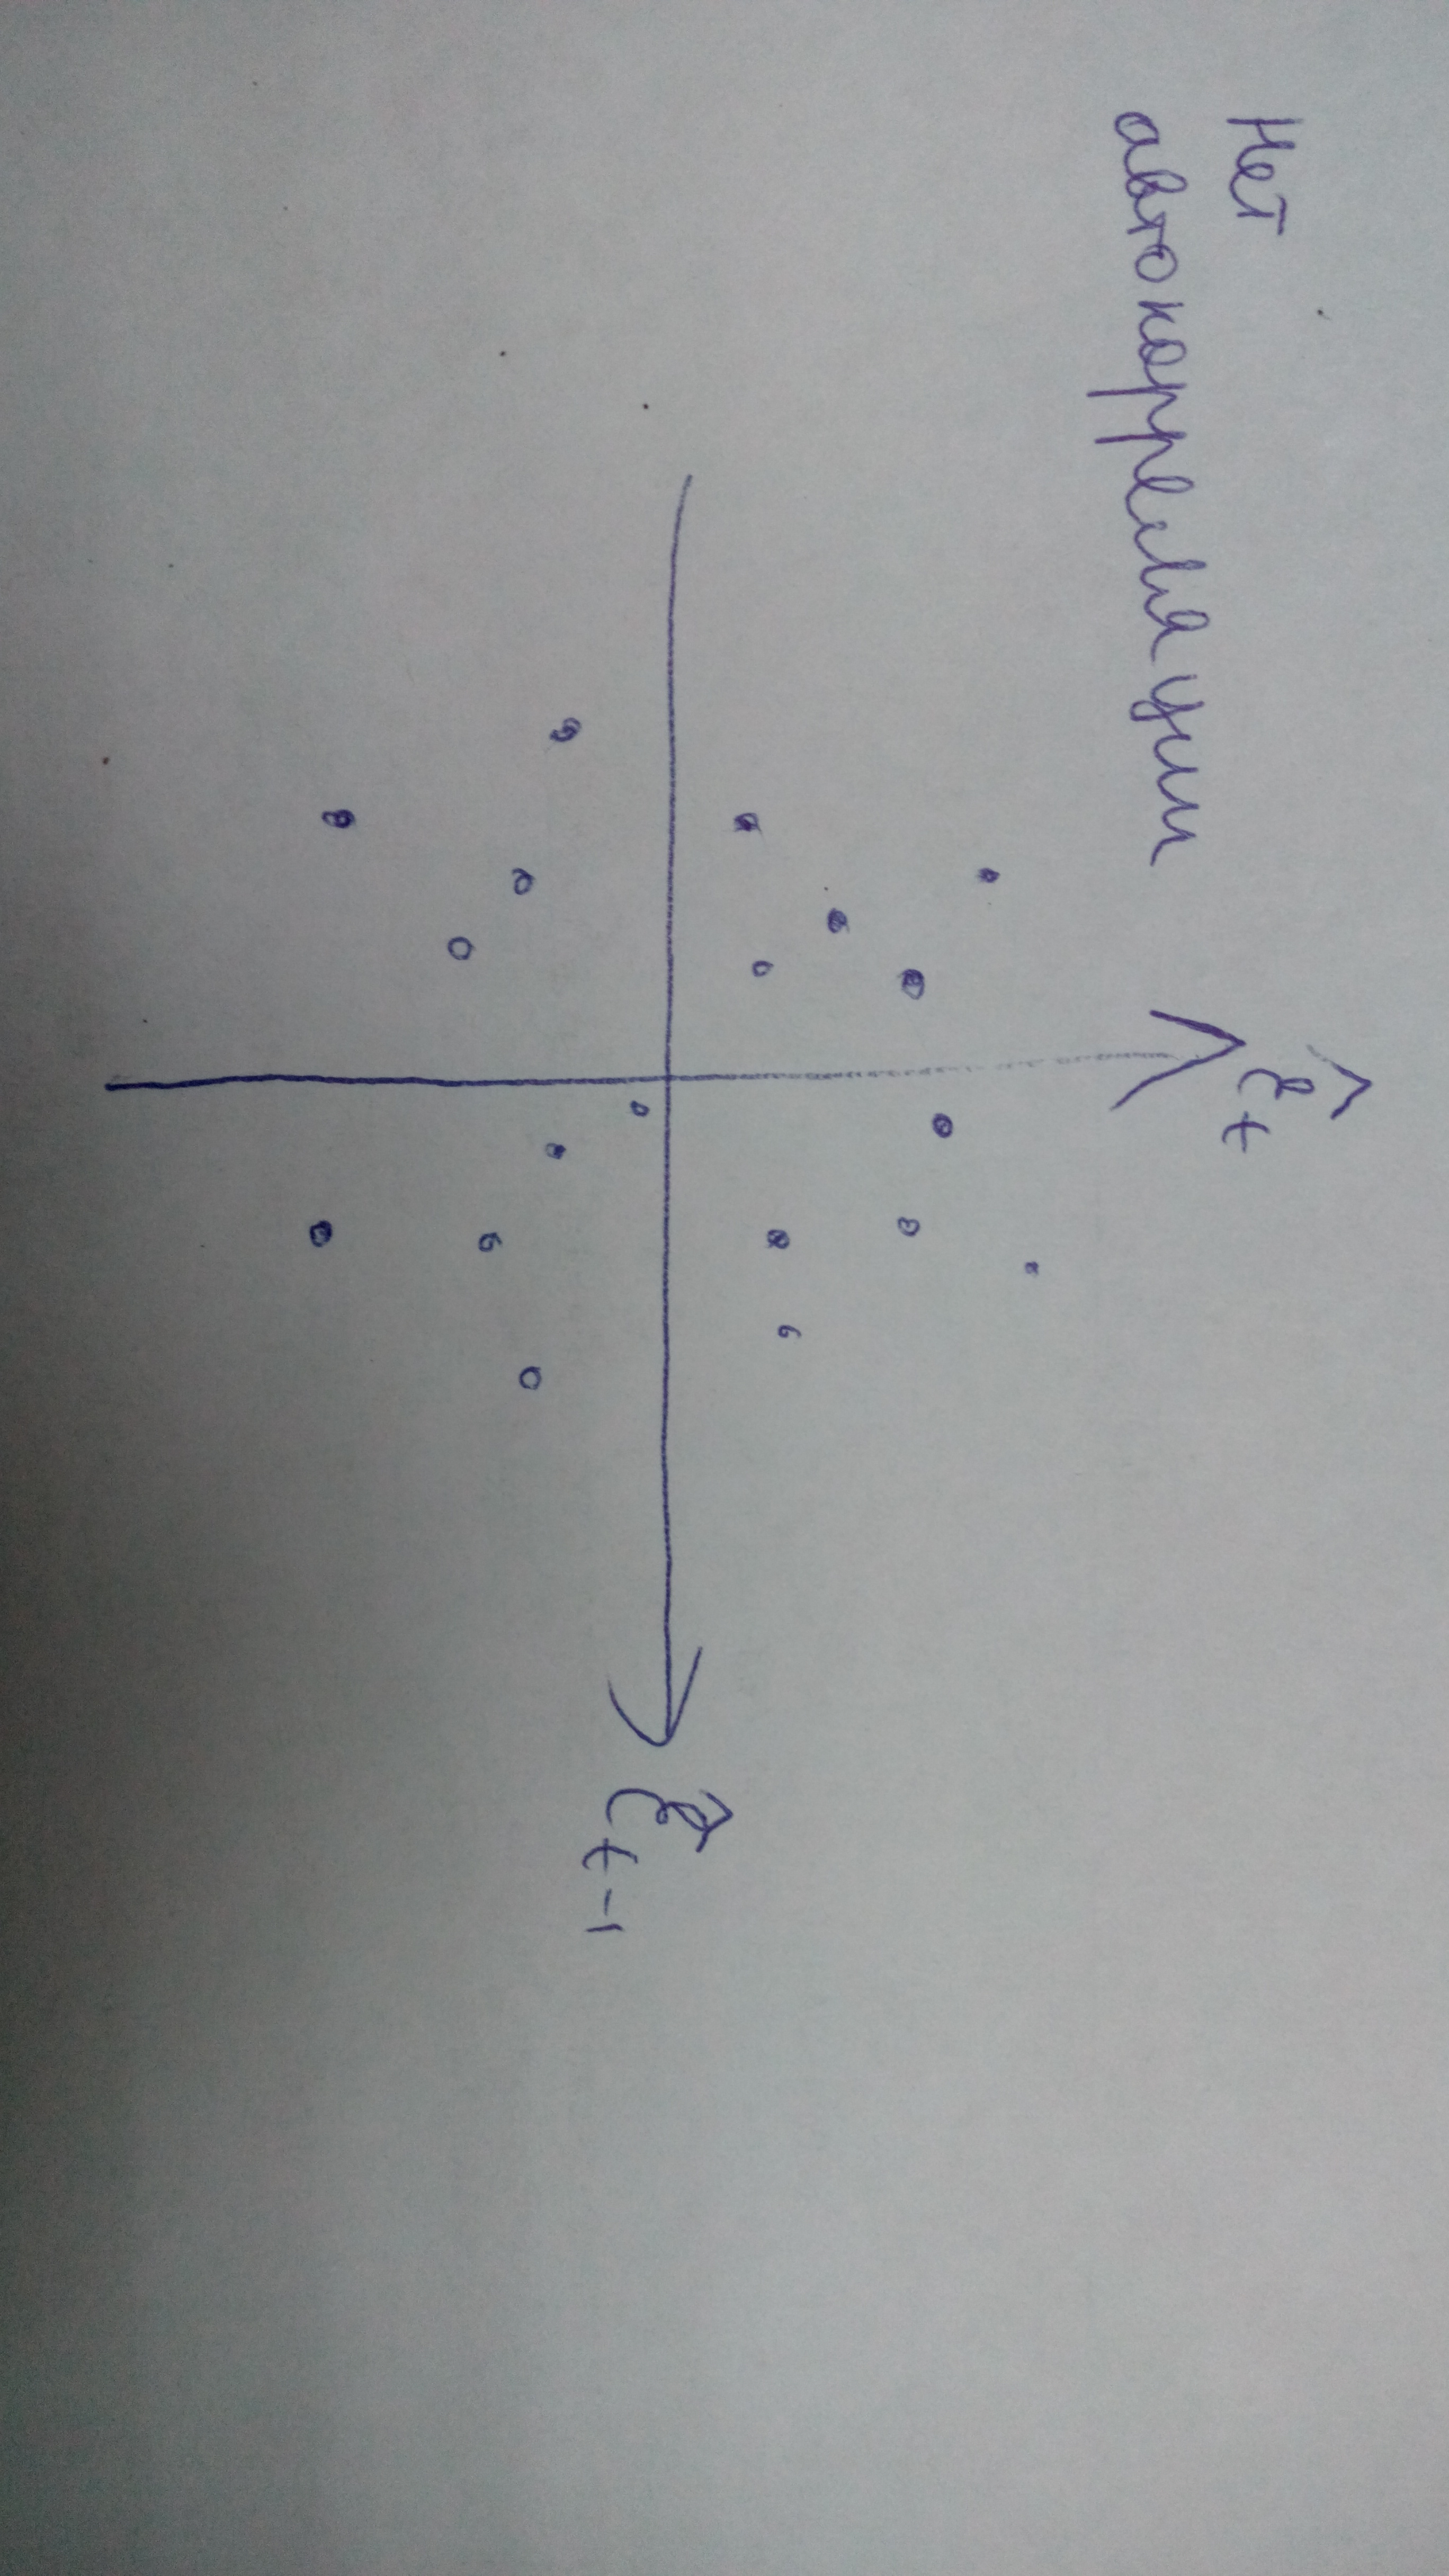
\includegraphics[scale=0.05, angle=90]{autocorr_0.jpg} 

4:31 график сменяется на

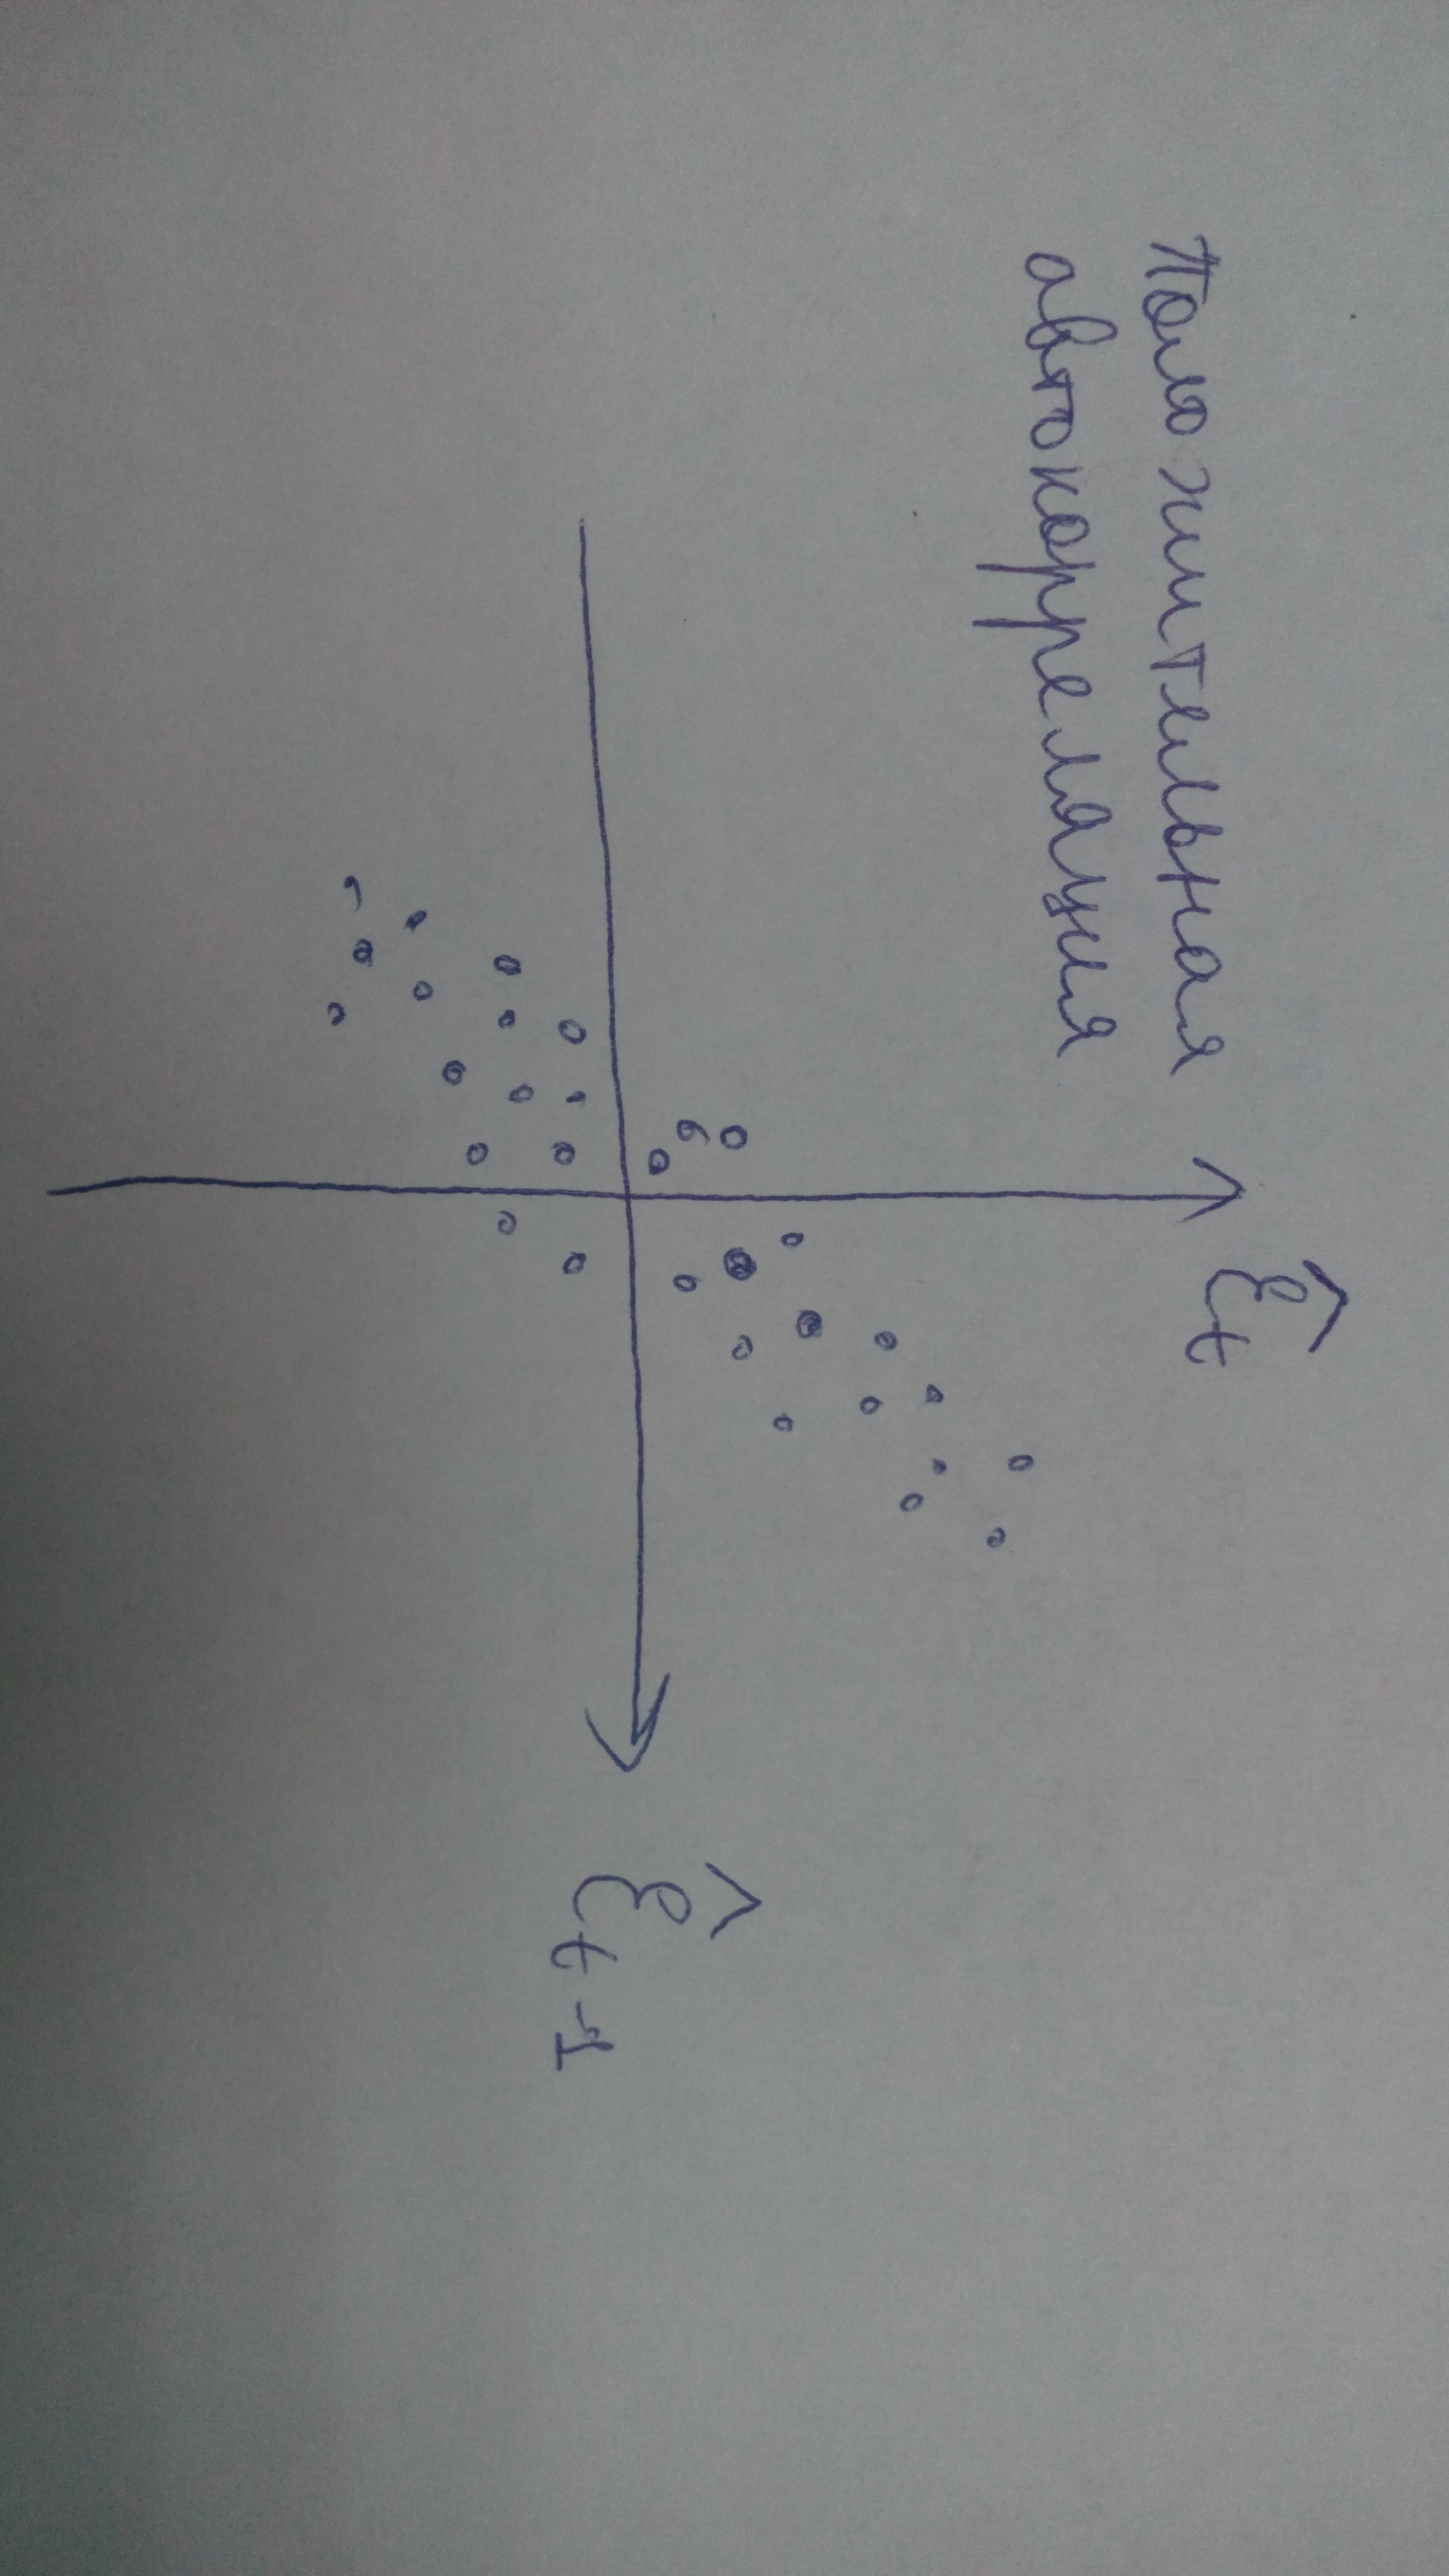
\includegraphics[scale=0.05, angle=90]{autocorr_1.jpg} 

4:47  график сменяется на 

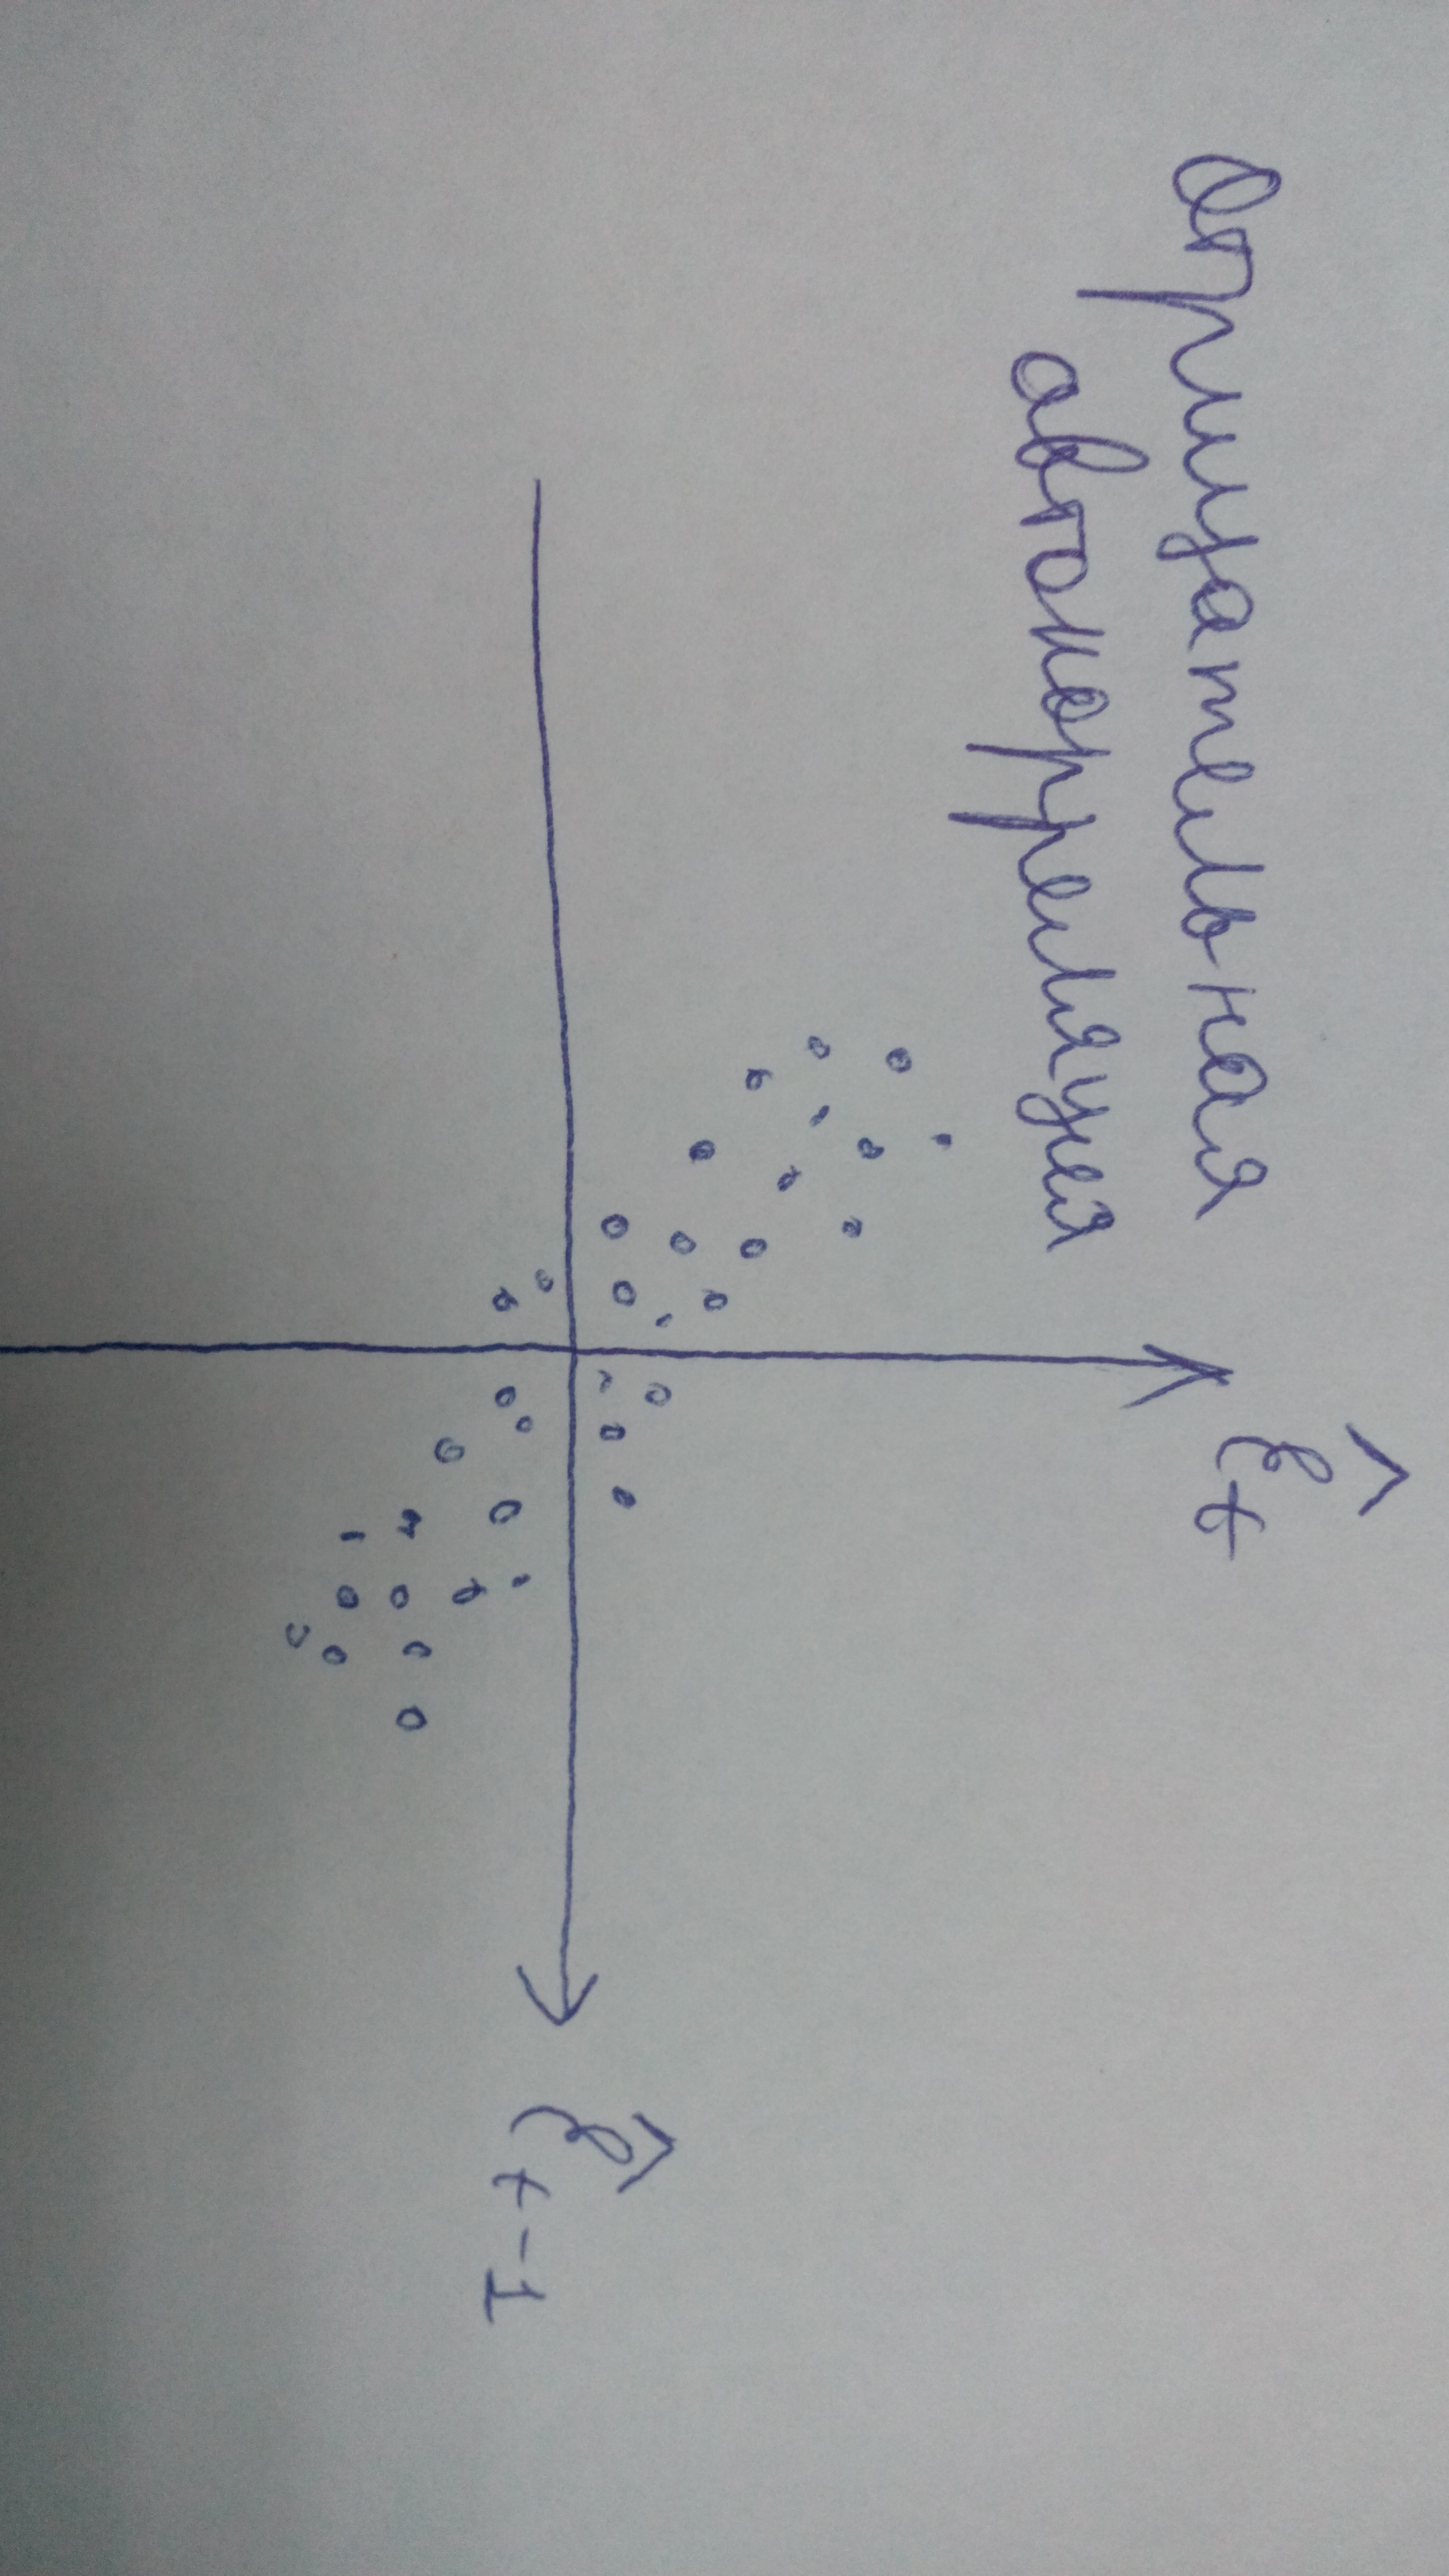
\includegraphics[scale=0.05, angle=90]{autocorr_m1.jpg} 

для монтажера: у всех графиков горизонтальная ось --- $\hat{\e}_{t-1}$, вертикальная ось --- $\hat{\e}_{t}$


5:41 исправляем первый пункт на

* автокорреляция первого порядка

$\e_t=\rho \e_{t-1}+u_t$

6:18 изменяем заголовок слайда на 

Тест Дарбина-Уотсона, алгоритм

7:41 исправляем третий пункт на

* $DW\approx 4$ означает отрицательную автокорреляцию $\hat{\rho} \approx -1$

8:07 добавляем ниже подписи:

* Если $P$-значение больше уровня значимости $\alpha$, то $H_0$ об отсутствии автокорреляции не отвергается

* Если $P$-значение меньше уровня значимости $\alpha$, то $H_0$ об отсутствии автокорреляции отвергается

6-1-5 Тест Бройша-Годфри. Пример тестирования автокорреляции

\url{http://www.youtube.com/watch?v=5XCeTZi3efk}

0:07 убираем <<кафедра публичной политики>>

0:16 изменить название видеофрагмента (на синей полосе внизу) на <<Тест Бройша-Годфри. Пример тестирования автокорреляции.>>

0:26 во фразе <<... порядка $p$ в ошибках...>> выделить букву $p$ синим 

2:14 оставляем заголовок слайда <<Процедура теста Бройша-Годфри>> и заменяем всё остальное на график

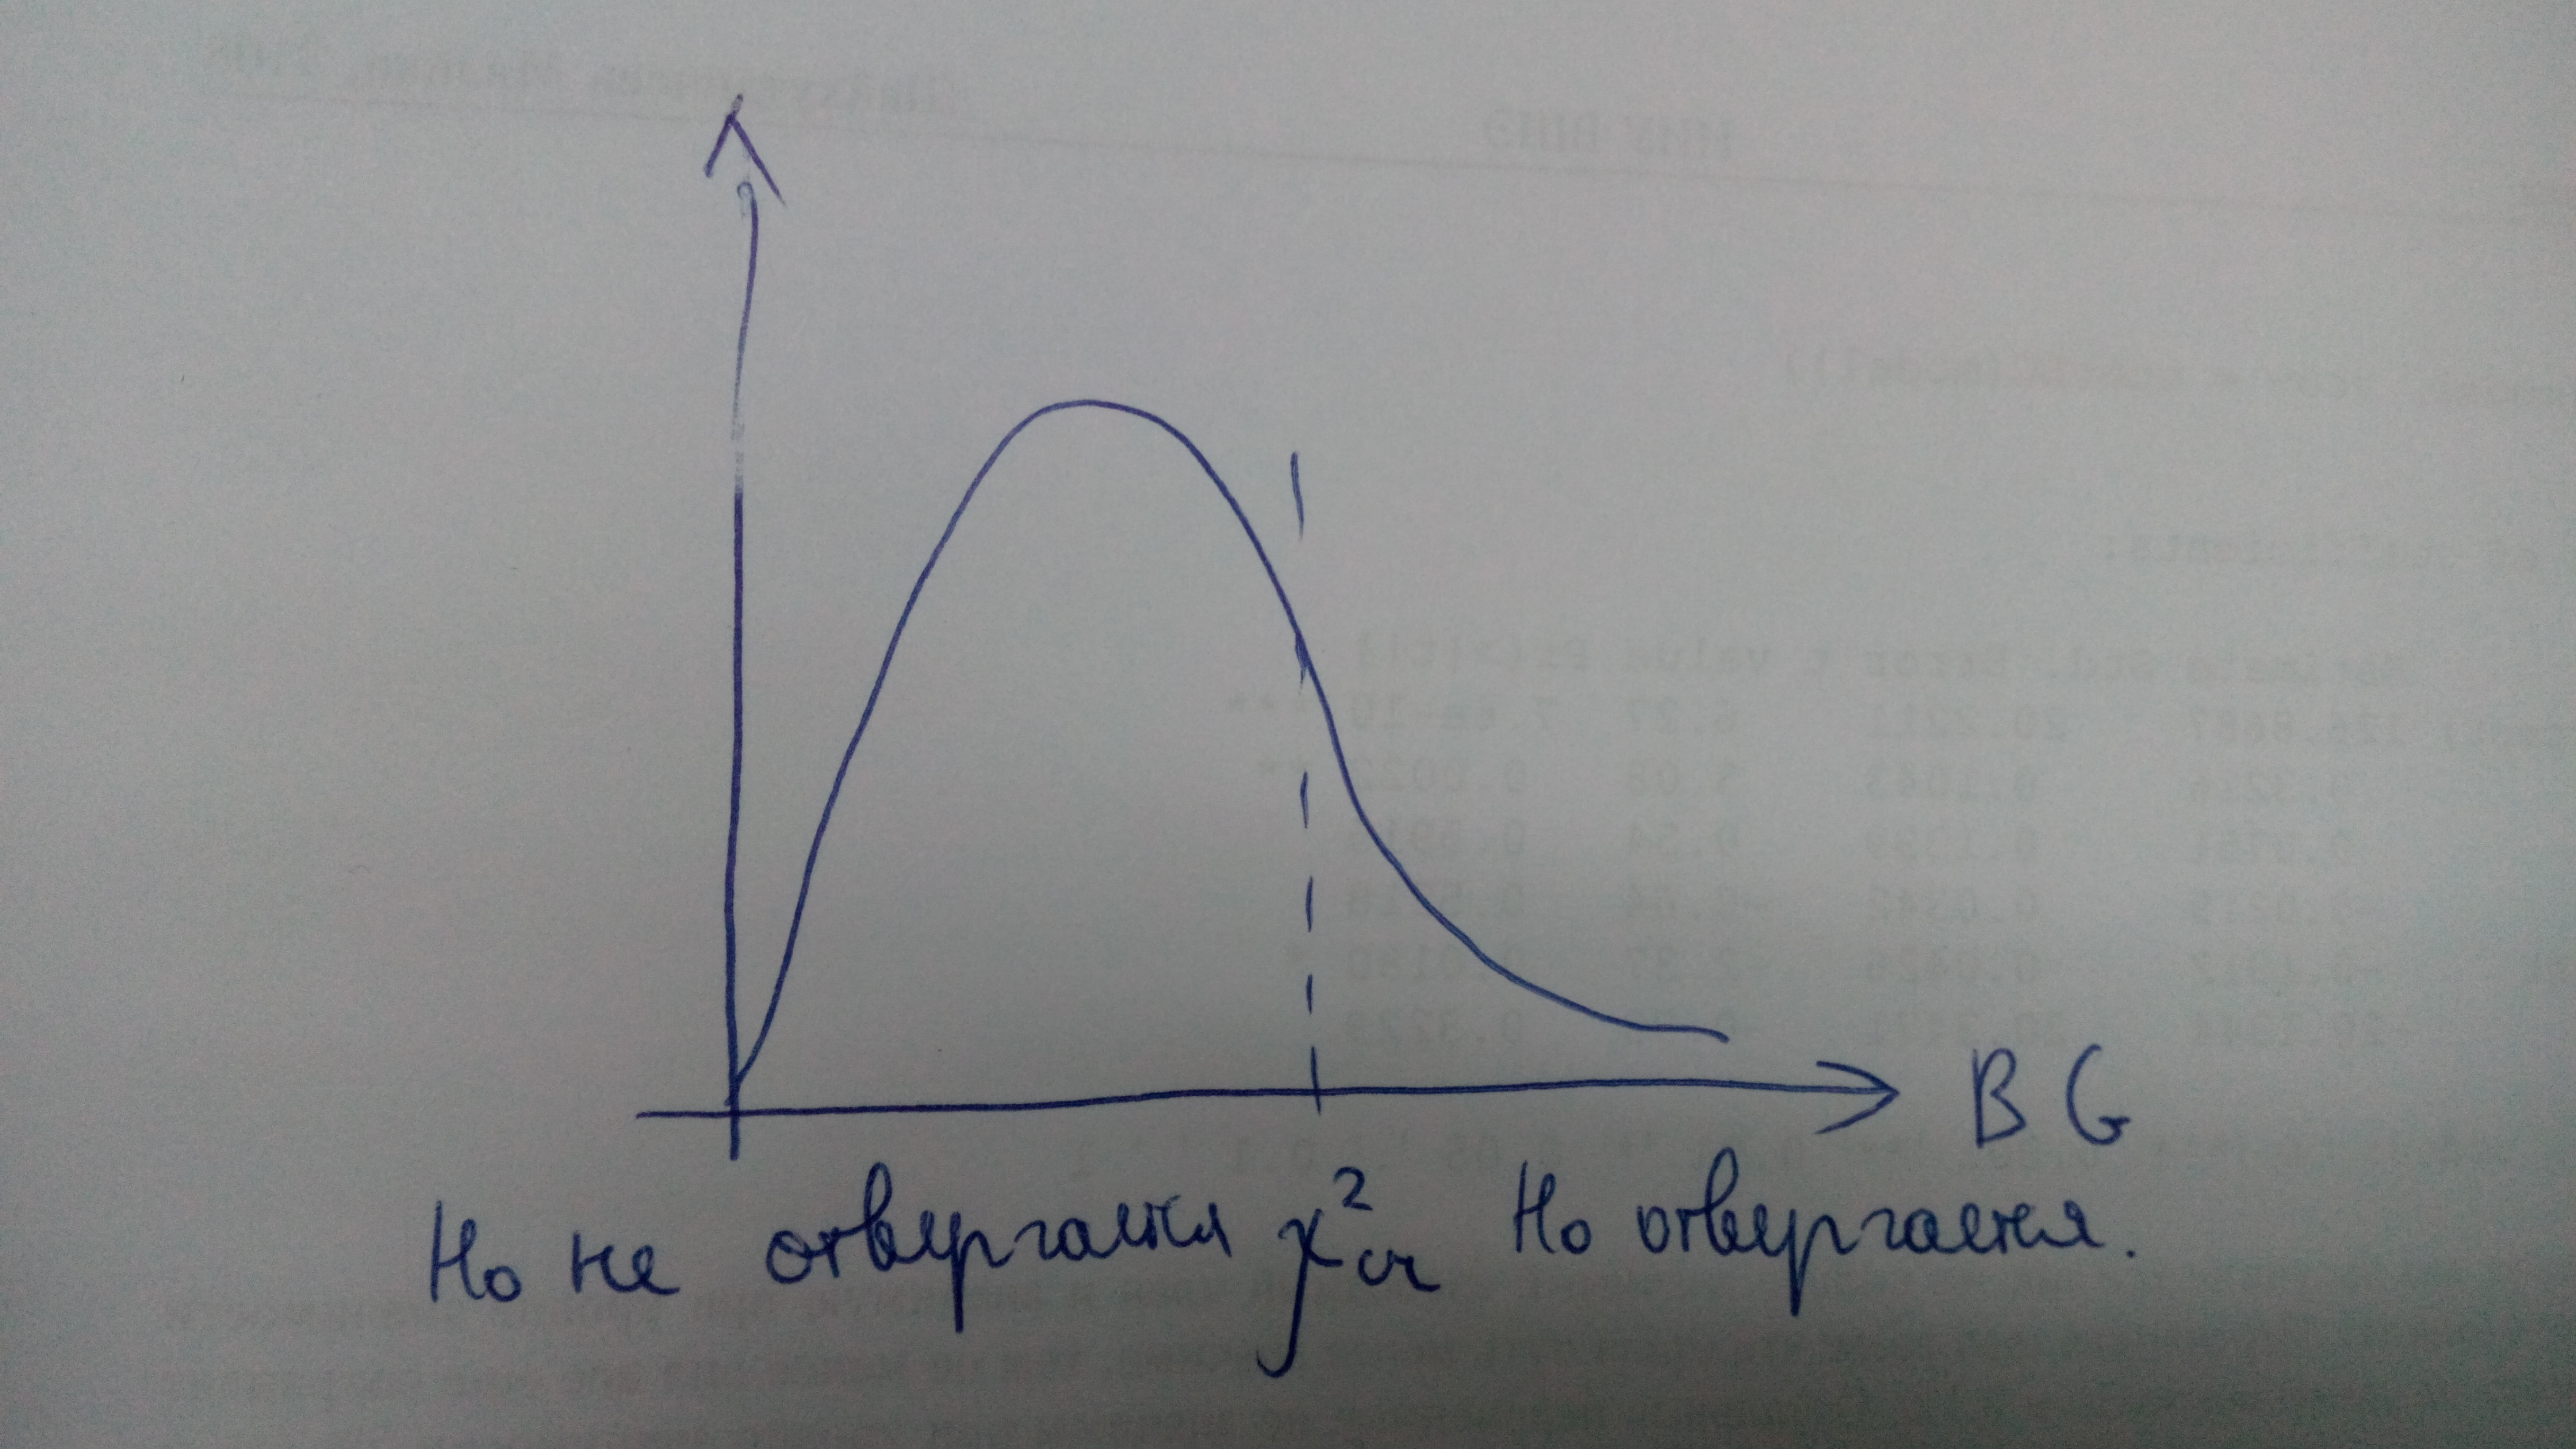
\includegraphics[scale=0.05, angle=0]{bg_test.jpg} 

для монтажера: ось называется $BG$, 

для монтажера: под осью написано: 

$H_0$ не отвергается \; $\chi^2_{cr}$ \; $H_0$ отвергается

3:12---4:13 статичная фотка ??? вырезать полностью 

4:20---5:13 ускорить --- я специально молча писал на доске условие задачи, чтобы оно потом было ускорено



6-2-1 Работа с датами в R

\url{http://www.youtube.com/watch?v=wDQriAxT_4E}

0:07 убираем <<кафедра публичной политики>>


6-2-2 Базовые действия с временными рядами

\url{http://www.youtube.com/watch?v=kTmEBWWN68Y}

0:07 убираем <<кафедра публичной политики>>


6-2-3 Загрузка данных из внешних источников

\url{http://www.youtube.com/watch?v=hszXyt1nt4w}

0:07 убираем <<кафедра публичной политики>>

7:48---8:16 вырезать и удалить

в конце подклеить кусок 0:16-0:33 из следующего фрагмента 

6-2-4  Построение робастных доверительных интервалов

\url{http://www.youtube.com/watch?v=O8aX-AU4KiA}

0:07 убираем <<кафедра публичной политики>>

кусок 0:16-0:33 вырезать и подклеить к концу фрагмента 6-2-3

8:36-8:59 вырезать 

9:17-9:22 вырезать

10:13-11:21 вырезать

6-2-5 Тесты на автокорреляцию

\url{http://www.youtube.com/watch?v=63HbND96rIQ}

0:07 убираем <<кафедра публичной политики>>

5:48-до конца вырезать и удалить

6-1-41 лишний фрагмент (копия 6-1-4), убрать совсем

\url{http://www.youtube.com/watch?v=A0CdRimMEHw}



\end{document}